\section{DESIGN}
\label{ch:design}

%為了自動化地探索可能的選項、選項參數，提出一種新的多參數模糊測試設計。首先，結合靜態分析、動態分析，找出目標程式中可用的選項並合理地組合。
%接著，利用污染源推論，針各個選項的選項參數進行分析，根據推論的結果變異選項參數。
%同時，改良模糊測試工具的 forkserver，使其能夠在不關閉重起的情況下，替換目標程式使用的參數。
%此架構根據執行階段提供的回饋，動態地調整選項的組合、選項參數的值，因此稱為選項感知模糊測試（Option-Aware Fuzzing）。
To automate the exploration of possible options and optional arguments, a novel multi-argument fuzzing design is proposed. First, by combining static and dynamic analysis, available options in the target program are identified and rationally combined.
Next, using taint inference, the arguments for each option are analyzed, and the arguments are mutated based on the inference results.
Simultaneously, the forkserver of the fuzzing tool is improved so that it can replace the parameters used by the target program without shutting down and restarting.
This architecture dynamically adjusts the combination of options and the values of arguments based on feedback provided during the execution phase, called Option-Aware Fuzzing.
%我們設計並實作了對應的開源原型：KOFTA。

\subsection{Option Analysis} %選項分析

%選項在原始碼中已經確定不變，因此編譯階段的靜態分析適用於尋找可用的選項。並且，只需要分析常用於解析參數的函式(例如 \texttt{strcmp()}、\texttt{getopt()}、\texttt{getopt\_long()})。
Since the options are fixed in the source code, static analysis during the compilation phase is only needed to find the available options. Furthermore, only functions commonly used to parse parameters (e.g., \texttt{strcmp()}, \texttt{getopt()}, \texttt{getopt\_long()}) need to be analyzed.

%一個專案中可能包含多個可執行檔 (例如 GNU Binutils 中包含了多個分析處理二進制檔案的工具：objdump、ar、ranlib 等)，也不一定會提供個別編譯的步驟[如 Binutils 就無法單獨編譯 objdump（未紀錄於相關文件中）]，必須連同其他工具。此時靜態分析的結果將無法確定特定選項應屬於哪一個執行檔。因此，需透過蒐集執行的回饋，動態分析正確可用的選項組合。

\subsubsection{Static Analysis} %靜態分析
\label{subsec:optana-static}

%在 C 標準函式庫中， \texttt{getopt()} 用於分析短選項：\texttt{optstring} 所含字串會描述可用的短選項，是分析的重點。
In the C standard function library, \texttt{getopt}(argc, *argv[], *optstring) is used to analyze short options: the string contained in \texttt{optstring} describes the available short options and is the focus of the analysis.
\iffalse
\begin{lstlisting}[numbers=none]
int getopt(int argc, char * const argv[],
           const char *optstring);
\end{lstlisting}
\fi
\iffalse
\begin{lstlisting}[numbers=none]
"abc:d::"
\end{lstlisting}
\else
"abc:d::",
\fi
%這個 \texttt{optstring}，描述了 \texttt{a}、\texttt{b}、\texttt{c}、\texttt{d} 四個短選項，選項字元後可接零至二個「 \texttt{:} 」代表該選項的「選項參數必要性」。
this \texttt{optstring} describes four short options \texttt{a}, \texttt{b}, \texttt{c}, and \texttt{d}. The option character can be followed by zero or two "\texttt{:}" to indicate the "optional argument necessity".
%零個「\texttt{:}」代表該選項單獨使用，「無」選項參數；一個「\texttt{:}」代表選項參數為「必要」，不可單獨使用；兩個「\texttt{:}」則代表選項參數「非必要」，選項可以單獨使用。

%對於長選項而言，GNU 標準的擴充（extension）提供
For long options, GNU standard extension provides
\iffalse
\begin{lstlisting}[numbers=none]
int getopt_long(int argc, char * const argv[],
                const char *optstring,
                const struct option *longopts,
                int *longindex);
\end{lstlisting}
\else
\texttt{getopt\_long}(argc, *argv[], *optstring, *longopts, *longindex).
\fi
%函式的前三個參數與 \texttt{getopt()} 相同，\texttt{optstring} 可用於分析短選項。
The first three parameters of the function are the same as those of \texttt{getopt()}, and \texttt{optstring} can be used to parse short options.
%第四個參數\texttt{longopts}描述可用的長選項，是一個結構陣列（structure array），陣列中每個項目是一個結構 (struct option)：
The fourth parameter, \texttt{longopts}, describes the available long options and is a structure array where each item is a struct option:
%\newpage
\iffalse
\begin{lstlisting}[numbers=none]
struct option {
    const char *name;
    int         has_arg;
    int        *flag;
    int         val;
};
\end{lstlisting}
\else
\{ *name; has\_arg; *flag; val;\}.
\fi
%第一個成員 \texttt{name} 是長選項的名稱；第二個成員 \texttt{has\_arg} 代表選項的「選項參數必要性」，同樣分為「無」、「必要」、「非必要」；第四個成員是一整數，若該整數位於 ASCII 的可視字元區間，經常代表長選項對應的短選項。
The first member \texttt{name} is the name of the long option; the second member \texttt{has\_arg} represents the "necessity of the optional argument", which is also divided into "none", "necessary" and "non-necessary"; the fourth member is an integer. If the integer is located in the visible character range of ASCII, it often represents the short option corresponding to the long option.

%除此之外，有一些程式單純使用「字串匹配」的方式實現命令列參數解析（如 Listing \ref{lst:xmllint-argparse}）。因此，分析\texttt{strcmp()} 的字串參數是否以「\texttt{-}」開頭，也有助於尋找可用的選項。
In addition, some programs simply use "string matching" to parse command-line arguments. Analyzing whether the string arguments of \texttt{strcmp()} begin with "\texttt{-}" can also help in finding available options.

%在編譯階段，透過分析\texttt{optstring}、\texttt{longopts}、\texttt{strcmp()}的字串參數，便能從原始碼中提取可用的選項，以及「選項參數必要性」。在這階段，透過\texttt{strcmp()}找到的選項，暫時無法確定「選項參數必要性」，須先標記為「非必要」。
%During the compilation phase, by analyzing the string arguments of \texttt{optstring}, \texttt{longopts}, and \texttt{strcmp()}, usable options and their "argument necessity" can be extracted from the source code. The "argument necessity" of the options found through \texttt{strcmp()} cannot be determined temporarily and must be marked as "non-necessary".

\subsubsection{Option Combination} %選項組合

%目標程式編譯時，可能需連同專案中其他的執行檔一起編譯。然而，可執行檔間往往會共用部份的原始碼檔案。
When compiling the target program, it may need to be compiled along with other executables in the project. However, executables often share some source code files.
%例如 GNU Binutils 中的 ar 和 ranlib 編譯時都需要 ar.c 這份原始碼，因此靜態分析時從 ar.c 中提取的選項，將無法確定應該屬於 ar 或是 ranlib。
%為了解決這個問題，分析 \texttt{strcmp()}、 \texttt{getopt()}、 \texttt{getopt\_long()} 等關鍵函式的同時，會生成一個隨機的識別碼。並在該關鍵函式呼叫處（call site）前插樁，用於執行時回報該識別碼。
To address this issue, a random identifier is generated while analyzing critical functions such as \texttt{strcmp()}, \texttt{getopt()}, and \texttt{getopt\_long()}. An instrument (\texttt{\_\_kofta\_optana(x)}) is then inserted before the call site of this critical function to report this identifier during execution.

%如同範例（Listing \ref{lst:optana-instrument}）所示，分析 \texttt{getopt()} 的同時會產生一個隨機的識別碼：\texttt{23927}，並將該識別碼作為函式 \texttt{\_\_kofta\_optana()} 的參數，插樁在 \texttt{getopt()} 之前呼叫。實際執行目標程式時，\texttt{\_\_kofta\_optana()} 會紀錄所有呼叫過的識別碼，被紀錄的識別碼會作為執行階段的回饋。KOFTA 會根據動態分析蒐集的識別碼搜尋靜態分析中對應的可用選項；在這個範例中，目標程式執行後 KOFTA 會根據識別碼 \texttt{23927} 找到 \texttt{-n} 及 \texttt{-t} 兩個可用選項，後續就可以組合這些選項產生下一次的測試。

%這項設計同時帶來了另一個好處：可以提高選項組合的合法機率。考慮一個巢狀的參數解析（Listing \ref{lst:optana-nested}），只有當第一個參數是 \texttt{--foo} 時，第二個參數 \texttt{--bar} 作為選項才有意義。
This design also brings another benefit: it increases the probability of valid option combinations (consider a nested argument parsing where the second parameter, \texttt{--bar}, is only meaningful as an option if the first parameter is \texttt{--foo}). It describes the dependencies between options, improving testing efficiency.
%設想在第一次不帶任何參數的測試執行後，KOFTA 會根據執行階段回饋的識別碼 \texttt{62376} 產生帶有 \texttt{--foo} 的下一組測試；帶有 \texttt{--foo} 參數的測試在執行階段將回饋兩個識別碼：\texttt{62376} 與 \texttt{11514}，因此下一組衍生的測試參數可能是 \texttt{--foo --foo} 或是 \texttt{--foo --bar}，後者可以順利進入巢狀結構的最內層，只有前者將是一次冗餘的測試。相較於過去研究中使用的參數組態檔，其無法描述選項之間的相依性，即使在沒有 \texttt{--foo} 選項的情況下，仍然可能產生很多包含 \texttt{--bar} 選項的測試，這些測試都將是無效而且浪費時間的；這個設計將提昇選項組合的測試效率。

%\vfill
\iffalse
\begin{lstlisting}[float=h!, caption=選項動態分析插樁範例, label=lst:optana-instrument]
int main(int argc, char** argv) {

    __kofta_optana(23927);
    while ((opt = getopt(argc, argv, "nt:")) != -1)
    {
        // ...
    }

}
\end{lstlisting}

\begin{lstlisting}[float=h!, caption=巢狀參數解析範例, label=lst:optana-nested]
int main(int argc, char** argv) {

    __kofta_optana(62376);
    if (!strcmp(argv[0], "--foo"))
    {
        __kofta_optana(11514);
        if (!strcmp(argv[1], "--bar"))
        {
            // ...
        }
    }

}
\end{lstlisting}
\fi
\subsubsection{Assessment for Optional Argument Necessity} %選項參數必要性評估

%與過去相關研究最大的不同在於：透過污染源分析的方法探索選項參數廣闊的輸入空間，因此確認一個選項是否能夠帶有選項參數至關重要。
%「選項參數必要性」分為三類：無、必要、非必要。「非必要」的選項參數通常代表存在預設值（default value），當該選項不帶選項參數、單獨使用時，選項參數的預設值便是實際使用值。
The biggest difference from past research lies in exploring the broad input space of optional arguments through taint analysis. Therefore, confirming whether an option can have optional argument is crucial.
"Optional argument necessity" is divided into three categories: none, necessary, and non-necessary. "non-necessary" arguments typically represent a default value. When the option is used alone without option argument, the default value of the argument is the actual value used.
%然而，不帶選項參數（就無法使用污染源分析）、只使用預設值（會失去探索其他路徑的機會），對於覆蓋率導向的模糊測試而言是不利的。因此， KOFTA 對於「非必要」的選項參數會更傾向於使其「必要」（也就是為該選項帶入參數），探索更多可能的執行路徑。
%在靜態分析階段中，由於無法確認藉由分析 \texttt{strcmp()} 所提取的選項參數必要性，因此會先將其標記為「非必要」（\S \ref{subsec:optana-static}）；即使是透過分析 \texttt{optstring} 或 \texttt{longopts} 找到的選項，標記為「非必要」選項參數，在解析時也可能實際是「無」。
During the static analysis phase, since the necessity of the optional arguments extracted by analyzing \texttt{strcmp()} cannot be confirmed, they are marked as "non-necessary" (\S \ref{subsec:optana-static}). Even if the option is found by analyzing \texttt{optstring} or \texttt{longopts} and marked as "non-necessary", it may actually be "none" during parsing.
%如同範例（Listing \ref{lst:optional-arg}）所示，靜態分析後可以知道「 \texttt{--disassemble} 」的選項參數必要性為「非必要」（\texttt{optional\_argument}），然而 objdump 在解析時卻將其視為一個「無」選項參數的選項（Line 13-17）。
%由此可見，貿然地將「非必要」皆視為「必要」是不可行的，必須有一個方法:蒐集執行階段回饋以評估選項參數必要性。
Therefore, it is not feasible to rashly regard all "non-necessary" as "necessary". There must be a method: collect feedback during the execution phase to evaluate the necessity of option arguments.

\iffalse
\begin{lstlisting}[float=h!, caption=\texttt{objdump} 非必要選項參數範例, label=lst:optional-arg]
static struct option longopts[]=
{
  {"disassemble", optional_argument, NULL, 'd'},
};

int main (int argc, char **argv)
{
  while ((c = getopt_long (argc, argv, optstring,
                           longopts, NULL)) != EOF)
  {
    switch (c)
    {
    case 'd':
      disassemble = true;
      disassemble_all = true;
      seenflag = true;
      break;
    }
  }
}
\end{lstlisting}

\begin{lstlisting}[float=h!, language=sh, caption=程式退出碼範例一, label=lst:exit-code-1]
$ objdump -d &> /dev/null 
$ echo $?                                
0
$ objdump -d xyz &> /dev/null
$ echo $?                                    
1
\end{lstlisting}
\fi

%要觀察使用的選項、選項參數是否合法，一個簡單的方法是檢查目標程式的退出碼（exit code）：慣例上，退出碼「 \texttt{0} 」表示程式正常執行；退出碼「非 \texttt{0} 」表示程式執行期間出現錯誤（Listing \ref{lst:exit-code-1}）。退出碼將作為執行階段的回饋交由 KOFTA 進行評估。
To check if the options and optional arguments used are valid, a simple method is to check the target program's exit code: by convention, "\texttt{0}" indicates that the program executed normally; "not \texttt{0}" indicates that an error occurred during program execution. The exit code will be submitted to KOFTA for evaluation as feedback during the execution phase.

\iffalse
針對「非必要」的選項參數，評估其選項參數必要性的方法主要分為三個階段。

第一階段會將「\texttt{0}」作為該選項的選項參數填充值進行測試，例如要測試的選項為「\texttt{-d}」便會產生「\texttt{-d 0}」。當測試執行後會檢查目標程式的退出碼，如果退出碼為「\texttt{0}」代表目標程式順利執行，便會將該選項的選項參數必要性重新標記為「必要」並結束評估；然而當退出碼為「非 \texttt{0}」時，並不一定代表該選項不能帶有選項參數，有可能是因為帶入的填充值「\texttt{0}」本身不是一個合法的選項參數。如同範例（Listing \ref{lst:exit-code-2}）所示，選項「\texttt{-m}」本身可以帶有選項參數，執行「\texttt{-m i386}」後的退出碼為 \texttt{0}；而「\texttt{xyz}」並非選項「\texttt{-m}」的合法選項參數，因此執行「\texttt{-m xyz}」後的退出碼不為 \texttt{0}。要評估這類選項的選項參數必要性需要進入下一個階段。

\iffalse
\begin{lstlisting}[float=h!, language=sh, caption=程式退出碼範例二, label=lst:exit-code-2]
$ objdump -d -m i386 &> /dev/null
$ echo $?                                        
0
$ objdump -d -m xyz &> /dev/null
$ echo $?                                        
1
\end{lstlisting}
\fi

第二階段會針對仍無法確定選項參數必要性的選項進行污染源推論，污染源推論的結果是一系列的「提示」，每個提示都有可能是該選項合法的選項參數之一（\S \ref{sec:args-explo}）。接著將提示逐一替換為選項參數的值進行測試。例如，對「\texttt{-m 0}」進行污染源推論後得到三個提示：\texttt{abc}、\texttt{i386}、\texttt{xyz}，便會逐一測試 \texttt{-m abc}、\texttt{-m i386} 與 \texttt{-m xyz}。一旦發現任何可用的選項參數（退出碼為 \texttt{0}），便會將該選項的選項參數必要性重新標記為「必要」並結束評估；反之需要進入第三個階段。

在最後一個階段中，會將選項不帶選項參數單獨進行測試，如果發現退出碼為 \texttt{0}，便會將該選項的選項參數必要性重新標記為「無」；反之則代表所有階段中的測試皆產生退出碼為非 \texttt{0} 的結果，這可能是因為與其他選項的組合不合法、或是與輸入檔的組合不合法，導致無法確定該選項的選項參數必要性，KOFTA 將維持其參數必要性不變、仍標記為「非必要」。

\fi

\subsection{Exploring Optional Arguments} %選項參數探索
\label{sec:args-explo}

%相比於選項，選項參數缺乏明顯的特徵，通常有更多的可能性，難以使用靜態分析直接從原始碼中提取。因此，本研究提出污染源推論 \cite{gan2020greyone}的方法：在執行階段找出選項參數可能的值作為「提示」回饋；同時探索提示與選項之間的關聯性，將選項與對應的選項參數進行合理的組合。
Compared to options, optional arguments lack obvious characteristics and usually have more possibilities, making them difficult to extract directly from the source code using static analysis. Therefore, this study proposes a taint inference method \cite{gan2020greyone}: during the execution phase, identify possible values of optional arguments as "hints"; simultaneously, explore the correlation between hints and options, and reasonably combine options with their corresponding arguments.

%過去污染源推論與模糊測試的研究中，為了講求分析的準確性，會捨棄所有不確定的結果(這對於選項參數的探索來說是不利的)。因此，本研究提出一種基於雜湊的折衷方法，犧牲部份的推論準確性、提昇選項參數探索的能力。
%In past studies on taint inference and fuzzing, all uncertain results were discarded in order to ensure analytical accuracy (which is detrimental to the exploration of optional arguments). Therefore, this study proposes a compromise method based on hashing, sacrificing some inference accuracy to improve the ability to explore optional arguments.

\subsubsection{Taint Inference} %污染源推論

%用於分析資料流，推論外部的輸入是否能夠影響程式執行時內部的記憶體。
Used to analyze data flows and infer whether external inputs can affect the internal memory during program execution.
%如果將選項參數設為「污染源」、分支條件設為「污染終點」，便能推論前者是否能影響後者。測試不同的選項參數是為了提高覆蓋率(有機會走訪不同的分支而產生新的執行路徑)。因此觀測選項參數如何影響特定分支條件成為了增加覆蓋率的關鍵。
If the optional argument is set as the "taint source" and the branch condition as the "taint sink," we can infer whether the former can affect the latter. Testing different option arguments is to improve coverage (by having the opportunity to visit different branches and generate new execution paths). %Therefore, observing how option arguments affect specific branch conditions becomes the key to increasing coverage.

%選項參數可以分為兩大類：字串與數值。字串相關的分支條件經常使用 \texttt{strcmp()} 來判斷該參數是否合法；數值相關的也會經由 \texttt{if-else} 檢查是否在合法的範圍。因此  \texttt{strcmp()} 的參數、 \texttt{if-else} 條件的運算元都可以考慮作為選項參數的「提示」。
Optional arguments can be divided into two main categories: string and number. String-related branch conditions often use \texttt{strcmp()} to determine the validity of the argument; number-related conditions are checked for validity using \texttt{if-else}. Therefore, the parameters of \texttt{strcmp()} and the operands of \texttt{if-else} conditions can both be considered as "hints".

%例如在範例（Listing \ref{lst:argparse-example}）中，與選項 \texttt{--foo} 相關的提示是 \texttt{if-else} 條件中的運算元「\texttt{100}」；與選項 \texttt{--bar} 相關的提示是 \texttt{strcmp()} 的參數「\texttt{xyz}」。根據這些提示， KOFTA 會產生 \texttt{--foo 99}、\texttt{--foo 100}、\texttt{--foo 101} 及 \texttt{--bar xyz} 等一系列的測試，嘗試通過這些分支條件。

\iffalse
\begin{lstlisting}[float=h!, caption=選項參數解析範例, label=lst:argparse-example]
  if (!strcmp(argv[i], "--foo"))
  {
    if (atoi(argv[i+1]) < 100)
    {
      // ...
    }
  }
  if (!strcmp(argv[i], "--bar"))
  {
    if (!strcmp(argv[i+1], "xyz"))
    {
      // ...
    }
  }
\end{lstlisting}
\fi

%要完成「污染源推論」:首先，需要在編譯階段對各個「污染終點」插樁；接著，透過這些插樁在執行階段蒐集執行路徑上污染終點的狀態。根據狀態為每個污染終點計算「雜湊」、紀錄為一個「節點」，多個節點串連成一個代表該執行路徑的「鏈結串列」（linked list）；若比較兩個鏈結串列，便可以知道兩路徑在何處發生分歧。
To complete the "taint inference": First, each "taint sink" needs to be instrumented during the compilation phase; then, the state of the taint sinks along the execution path is collected through these instrumentations during the execution phase. Based on the state, a "hash" is calculated for each taint sink and recorded as a "node". Multiple nodes are linked together to form a "linked list" representing the execution path; by comparing two linked lists, it can be determined where the two paths diverge.

%我們感興趣的污染終點除了 \texttt{strcmp()} 的字串參數、\texttt{if-else} 比較條件的運算元以外，還有 \texttt{switch-case} 的運算元及各個目標（case）的值。
In addition to the string parameters of \texttt{strcmp()} and the operands of \texttt{if-else} comparison conditions, the taint sinks we are interested in also include the operands of \texttt{switch-case} and the values of each target (case).

%如同範例（Listing \ref{lst:tntsnk-example}）所示，
%也就是, \texttt{strcmp()} 之前會有 \texttt{\_\_kofta\_trace\_str()} 插樁，兩者參數相同； \texttt{if-else} 之前會有 \texttt{\_\_kofta\_trace\_cmp()}，並將比較條件的左、右運算元作為參數； \texttt{switch-case} 之前會有 \texttt{\_\_kofta\_trace\_swt()}，第一個參數是目標的數量、第二個參數是包含所有目標的陣列、第三個參數是比較的運算元。 這三個插樁函式會根據傳入的參數計算雜湊值，形成一個新的節點至目前的鏈結串列中。
In other words, \texttt{strcmp()} is preceded by \texttt{\_\_kofta\_trace\_str()}, both with the same parameters;
\texttt{if-else} is preceded by \texttt{\_\_kofta\_trace\_cmp()}, which takes the left and right operands of the comparison condition as arguments;
\texttt{switch-case} is preceded by \texttt{\_\_kofta\_trace\_swt()}, where the first parameter is the number of targets, the second is the array containing all targets, and the third is the comparison operand.
These three instrumentation functions calculate a hash value based on the passed arguments, forming a new node in the current linked list.

\iffalse

\begin{lstlisting}[float=h!, caption=污染終點插樁範例, label=lst:tntsnk-example]
  __kofta_trace_str(argv[i], "i386");
  __kofta_trace_cmp(!strcmp(argv[i], "i386"), 0);
  if (!strcmp(argv[i], "i386"))
  {
    // ...
  }
  __kofta_trace_cmp(atoi(argv[i]), 100);
  if (atoi(argv[i]) < 100)
  {
    // ...
  }
  __kofta_trace_swt(2, {'x', 'y'}, argv[i][0]);
  switch (argv[i][0])
  {
    case 'x':
      // ...
      break;
    case 'y':
      // ...
      break;
  }
\end{lstlisting}

\fi

%考慮以下目標程式（Listing \ref{lst:tntana-exec-example1}）中，要對選項「\texttt{--kofta}」的選項參數進行污染源推論，至少需要執行目標程式兩次。假設第一次以「\texttt{--kofta foo}」執行，至少會在鏈結串列中產生四個節點：strcmp（Line 3）、ifcmp（Line 3）、ifcmp（Line 7）、ifcmp（Line 10），代表本次測試的執行路徑（Figure \ref{fig:tntana-exec-example1}）。接著第二次測試中，我們將選項「\texttt{--kofta}」的選項參數改變後以「\texttt{--kofta xyz}」執行，在這次測試的執行路徑中同樣會產生四個鏈結串列的節點；不同的是，從第三個節點開始與第一次執行的結果不同（Figure \ref{fig:tntana-exec-example2} 中靠左紅圈處）。因此我們可以推論：選項「\texttt{--kofta}」的選項參數「污染」了該節點的比較條件。而被污染節點上的運算元「\texttt{a}」將作為「提示」回饋，於是 KOFTA 可以根據提示產生「\texttt{--kofta a}」的測試、產生新的測試覆蓋率。

\subsubsection{Characteristic Value of Taint Sink} %污染終點特徵值
\label{subsec:tntana-chara}

%在範例（Figure \ref{fig:tntana-lnklst-example}）中，除了第三個節點以外，實際上第四個節點（Figure \ref{fig:tntana-exec-example2} 中靠右紅圈處）也是被污染的污染終點。
%在範例（Listing \ref{lst:tntana-exec-example1}）中，除了節點(\texttt{if (arg == 'a')})以外，節點（\texttt{else if (arg == 'b'）})實際上也是被污染的污染終點。
In the example (Listing \ref{lst:tntana-exec-example1}), in addition to the node (\texttt{if (arg == 'a')}), the node (\texttt{else if (arg == 'b')}) is also actually a tainted sink.

%然而，過去將污染源推論與模糊測試結合的研究中，認為一旦發現第一個被污染的污染終點，後續的污染終點將沒有參考價值。因為當比較條件的運算元改變，代表後續的執行路徑很有可能也發生改變，此時再去比較兩個鏈結串列的節點已經沒有意義。這樣的作法提高了污染源推論的準確性；但也捨棄了其他可能被污染的污染終點，無法在該範例（Listing \ref{lst:tntana-exec-example1}）中推論出「\texttt{--kofta b}」這個參數的組合。
However, past studies combining taint inference with fuzz testing have argued that once the first tainted sink is identified, subsequent taint sinks become meaningless. This is because changes in the operands of the comparison conditions likely alter the subsequent execution path, making comparisons of the nodes in two linked lists pointless. This approach improves the accuracy of taint inference but discards other potentially taint sinks, making it impossible to infer the combination of arguments "\texttt{--kofta b}" in this example (Listing \ref{lst:tntana-exec-example1}).
%
\iftrue

%\begin{lstlisting}[float=hb!, caption=污染源推論執行範例一, label=lst:tntana-exec-example1]
\begin{lstlisting}[float=h!, caption={\footnotesize Taint Inference Execution (Example 1)}, label=lst:tntana-exec-example1]
int mode = MODE_NONE;
if (!strcmp(argv[i], "--kofta")) {
  char arg = argv[i++][0];
  if (arg == 'a') {
    mode = MODE_A;
  }
  else if (arg == 'b') {
    mode = MODE_B;
  }
}
\end{lstlisting}

\fi
%\vfill

\iffalse

\begin{figure}[h!]
     \centering
     \begin{subfigure}[]{0.48\textwidth}
         \centering
         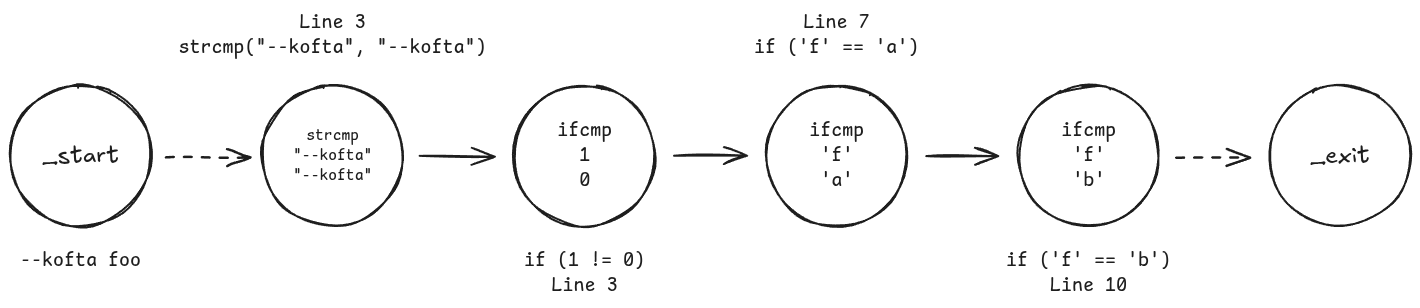
\includegraphics[width=\textwidth]{img/tntana-exec-example1.png}
%         \caption{測試 \texttt{--kofta foo} 產生的執行路徑}
         \caption{\footnotesize Execution Path of Testing \texttt{--kofta foo}}
         \label{fig:tntana-exec-example1}
     \end{subfigure}
     \begin{subfigure}[]{0.48\textwidth}
         \centering
         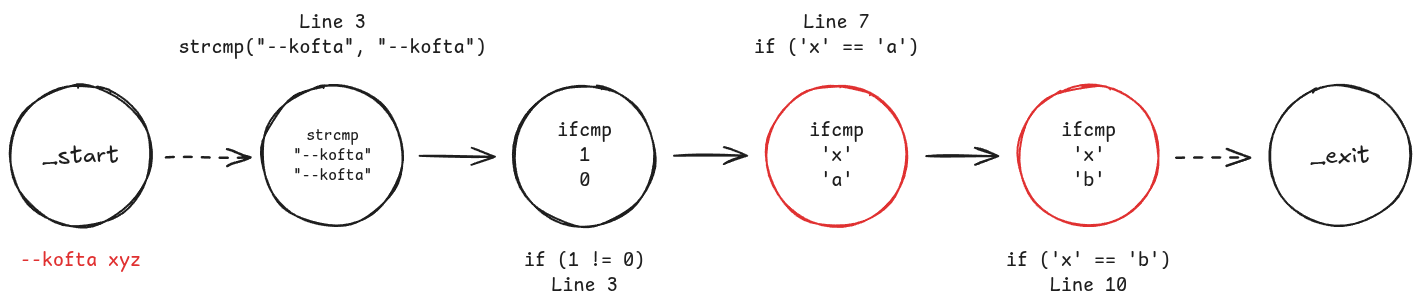
\includegraphics[width=\textwidth]{img/tntana-exec-example2.png}
%         \caption{測試 \texttt{--kofta xyz} 產生的執行路徑}
         \caption{\footnotesize Execution Path of Testing \texttt{--kofta xyz} }
         \label{fig:tntana-exec-example2}
     \end{subfigure}
%        \caption{污染源分析鏈結串列範例}
        \caption{Example: Linked List of Taint Analysis}
        \label{fig:tntana-lnklst-example}
\end{figure}

\fi

%\texttt{KOFTA} 提出加強方法判斷這種由 \texttt{if-else} 組成的「污染終點群組」。若群組中比較的對象相同（Line 7,10 皆比較 \texttt{arg}）則應將群組中比較條件的運算元（Line 7 的 \texttt{a} 與 Line 10 的 \texttt{b}）皆作為提示回饋。
KOFTA proposes an enchanced method to identify this "taint sink groups" consisting of \texttt{if-else} statements. If the objects being compared in the group are the same (both lines 7 and 10 compare \texttt{arg}), then the operands of the comparison conditions in the group (\texttt{a} in line 7 and \texttt{b} in line 10) should be given as feedback hints.

%為了判斷「污染終點群組」比較的對象是否相同，會根據該節點的「比較對象」與「污染終點類型（\texttt{strcmp()}、\texttt{if-else} 或 \texttt{switch-case}） 」計算一個雜湊值，稱為該污染終點的「特徵值」。
\texttt{To determine whether the objects compared in a "taint sink group" are the same}, a hash value is calculated based on the node's "comparison object" and "taint sink type (\texttt{strcmp()}, \texttt{if-else}, or \texttt{switch-case})", which is called the "\textbf{characteristic value}" of the tainted sink.
%換句話說，當兩個相同類型的污染終點之比較對象也相同時，兩個節點將會有相同的特徵值。
%
%在發現第一個被污染的污染終點時紀錄其特徵值，與後續相鄰的節點比較，如果兩兩特徵值相同(代表它們可能屬於同一個污染終點群組、且有相同的比較對象)，應將比較條件的運算元皆作為提示回饋（Figure \ref{fig:tntana-group-example}）；這個比較會持續到發現第一個特徵值不同的節點為止。
When the first tainted sink is found, its characteristic value is recorded and compared with the subsequent adjacent nodes. If the characteristic values are the same for all pairs of nodes (meaning they may belong to the same taint sink group and have the same comparison object), the operands of the comparison condition should be used as feedback hints. This comparison will continue until the first node with different characteristic values is found.

%\vfill
\iffalse

\begin{figure}[h!] %hb
    \centering
    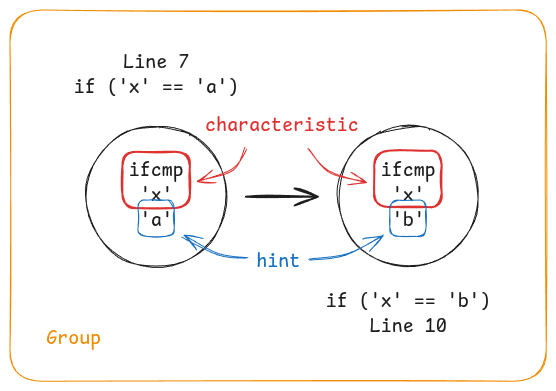
\includegraphics[width=0.4\textwidth]{img/tntana-group-example.png}
%    \caption{污染終點群組、特徵值、提示範例}
    \caption{\footnotesize Taink-Sink Group．Characteristic Value．Hint}
    \label{fig:tntana-group-example}
\end{figure}

\fi

\subsubsection{Non-Continuous Taint-Sink Group} %非連續污染終點群組

%在污染源推論中加上特徵值作為參考，雖然可能降低推論的準確性，但能提供更多潛在污染終點的提示，這對選項參數的探索是十分有利的。
Adding characteristic values as a reference to taint inference may reduce the accuracy of the inference, but it can provide more hints about taint sinks, which is very helpful for exploring optional arguments.
%然而，依 \ref{subsec:tntana-chara} 的設計只考慮一個污染終點群組內部的節點，仍然是不夠完整。
However, the design of \ref{subsec:tntana-chara} only considers nodes within a single taint sink group, which is still incomplete.

%試想以下的執行路徑 -- 鏈結串列（Figure \ref{fig:tntana-dscgrp-example}）：綠色圓圈與藍色圓圈的節點皆是被選項「\texttt{--kofta}」之選項參數污染的污染終點。其中，兩個相鄰的綠色圓圈有相同的特徵值，組成了污染終點群組並且可以被 \S \ref{subsec:tntana-chara} 中的方法識別；然而，藍色圓圈不僅沒有與綠色圓圈的污染終點群組相連，其特徵值也與綠色節點的不同。為了識別藍色圓圈的污染終點，需要額外的判斷。
Consider the following execution path -- a linked list (Figure \ref{fig:tntana-dscgrp-example}): Both the green and blue circles contain nodes that are tainted sinks by the optional argument of "\texttt{--kofta}" option. Two adjacent green circles share the same characteristic value, forming a taint sink group that can be identified by the method in \S \ref{subsec:tntana-chara}; however, the blue circle is not only not connected to the taint sink group of the green circles, but its characteristic value is also different from that of the green nodes. Additional judgment is needed to identify the taint sink of the blue circle.

\begin{figure}[h!] %ht
    \centering
    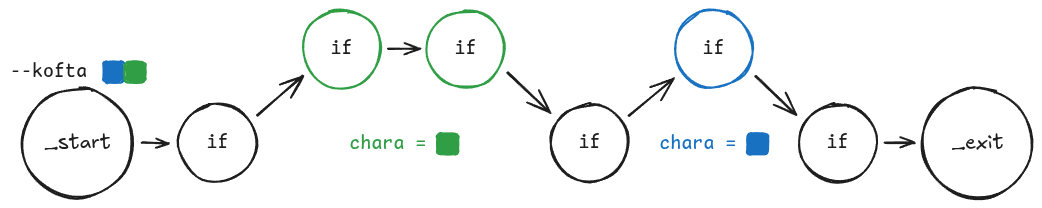
\includegraphics[width=0.48\textwidth]{img/tntana-dscgrp-example.png}
%    \caption{非連續污染終點群組範例}
    \caption{\footnotesize Non-Continuous Taint-Sink Group}
    \label{fig:tntana-dscgrp-example}
\end{figure}

%當污染終點群組結束後，可以比較下一個節點是否與原先鏈結串列中對應位置的節點相同。如果發現節點相同，可以視為前面被污染的節點的比較條件運算子雖然改變，但並因此未走訪不同的分支；既然仍在相同執行路徑上，便能夠繼續比較兩個鏈結串列中的節點是否相同。此時發現藍色圓圈的節點產生分歧，便將它視為一個新的污染終點群組，紀錄其特徵值與後續的節點做比較。
After the taint sink group ends, we can compare whether the next node is the same as the corresponding node in the original linked list. If the nodes are the same, it can be considered that although the comparison condition operand of the previously tainted node has changed, it has not visited different branches. Since it is still on the same execution path, we can continue to compare whether the nodes in the two linked lists are the same. At this point, a divergence is found in the node circled in blue, so it is regarded as a new taint sink group, and its characteristic value is recorded and compared with the subsequent nodes.

\subsection{Multi-Argument Forkserver}

\iffalse
除了「評估選項參數必要性」外，「探索選項參數」的方法也是建立於「污染源推論」上。「污染源推論」的原理是：觀察一個選項帶有不同的選項參數時，執行路徑上污染終點的狀態是否發生改變。由此可見，目標程式的命令列參數需由 forkserver 經常改變。若是每次「參數改變」都需要暫時關閉 forkserver，使用 exec 系統呼叫的額外成本將會相當可觀。因此，AFL的 forkserver 必須改良成：在不關閉的情況下，也能更換目標程式的命令列參數。
\else
Besides "evaluating the necessity of option arguments," the method of "exploring option arguments" is also based on "taint inference." The principle of which is to observe whether the state of the taint sink on the execution path changes when an option has different option arguments. Therefore, it is evident that the command-line arguments of the target program need to be frequently changed by the forkserver. If the forkserver needs to be temporarily shut down every time "arguments are changed," the additional cost of using the exec system call will be considerable. Therefore, AFL's forkserver must be improved so that the command-line arguments of the target program can be changed without shutting it down.
\fi

\subsubsection{Forkserver Principle}

\iffalse
其運作原理是在目標程式中，為「建構子（constructor）」函式增加了程式碼片段，如圖（Figure \ref{fig:afl-forkserver}）所示。目標程式在進入 \texttt{main()} 之前，還可呼叫許多其他函式進行初始化，包括由程式自定義的一系列建構子函式(forkserver 正是其中之一)。forkserver 在使用 \texttt{fork} 呼叫後，「子程序」會從 \texttt{forkserver} 返回，繼續執行剩餘的建構子函式，最終進入 \texttt{main()} 執行；「父程序」藉由迴圈留在 \texttt{forkserver} 中，等待下一次的 \texttt{fork} 呼叫。
\else
Its operating principle involves adding code snippets to the "constructor" functions \cite{Horgan2022} within the target program, hooked in \texttt{\_\_do\_global\_ctors\_aux()}. Before entering \texttt{main()}, the target program can call many other functions for initialization, including a series of user-defined constructor functions (forkserver is one of them). After forkserver is called using \texttt{fork}, the "child process" returns from \texttt{forkserver} and continues executing the remaining constructor functions, eventually entering \texttt{main()} for execution; the "parent process" remains in \texttt{forkserver} through a loop, waiting for the next \texttt{fork} call.
\fi

\iffalse
\begin{figure}[h!] %[hb]
    \centering
    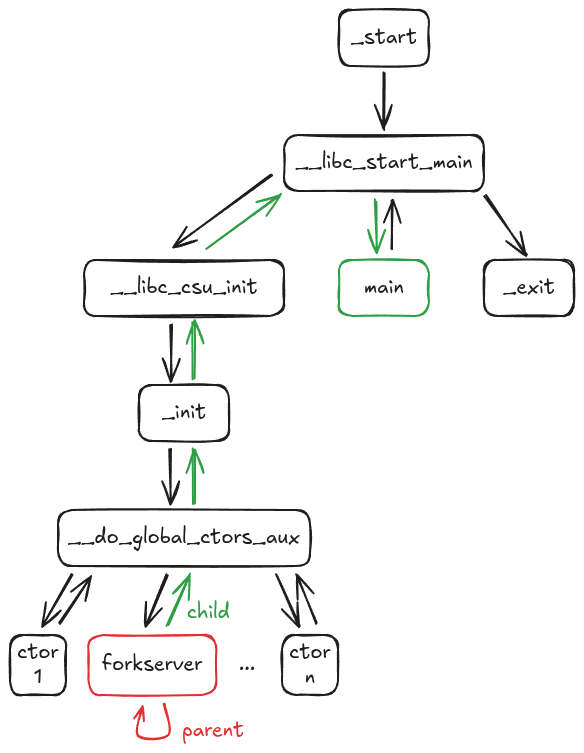
\includegraphics[width=0.4\textwidth]{img/forkserver.png}
    \caption{AFL forkserver}
    \label{fig:afl-forkserver}
\end{figure}

\fi

\subsubsection{Pointer Array for Multiple Arguments} % 命令列參數指標
\label{subsec:cmdln-argptr}

\iffalse
從流程圖（Figure \ref{fig:afl-forkserver}）中發現，\texttt{main()} 由 \texttt{\_\_libc\_start\_main()} 呼叫。因此，傳入的引數「\texttt{int argc}」與「\texttt{char *argv[]}」也應該位於記憶體堆疊（stack）上。再者，從 \texttt{\_\_libc\_start\_main()} 至 forkserver 的路徑單純，對於大部分的一般程式而言，由這條執行路徑產生的記憶體佈局（memory layout）應該皆相同；換言之，從 forkserver 的堆疊至位於 \texttt{\_\_libc\_start\_main()} 堆疊上「\texttt{argc}」與「\texttt{argv}」的記憶體位置偏移量（offset）應該是一固定值（Figure \ref{fig:fsrv-memlyt}），只因電腦環境不同而改變。紀錄並使用該偏移量正確找到 \texttt{argc} 與 \texttt{argv} 的位置後，便可在使用 fork 呼叫前，修改即將傳入 \texttt{main()} 的命令列參數，實現支援多參數之 forkserver。
\else
As seen in the start-up flowchart \cite{Horgan2022}, \texttt{main()} is called by \texttt{\_\_libc\_start\_main()}. Therefore, the passed-in arguments \texttt{int argc} and \texttt{char *argv[]} should also reside on the memory stack. Furthermore, the path from \texttt{\_\_libc\_start\_main()} to forkserver is simple, and for most general programs, the memory layout generated by this execution path should be the same. In other words, the memory offset from the forkserver stack to the memory locations of \texttt{argc} and \texttt{argv} on the \texttt{\_\_libc\_start\_main()} stack should be a fixed value (\texttt{Memory Layout}), changing only due to different computer environments. After recording and using this offset to correctly find the positions of \texttt{argc} and \texttt{argv}, the command-line arguments to be passed to \texttt{main()} can be modified before using the fork call, enabling forkserver to support multiple parameters.
\fi
%\vfill

\iffalse
\begin{figure}[h!] %[hb]
    \centering
    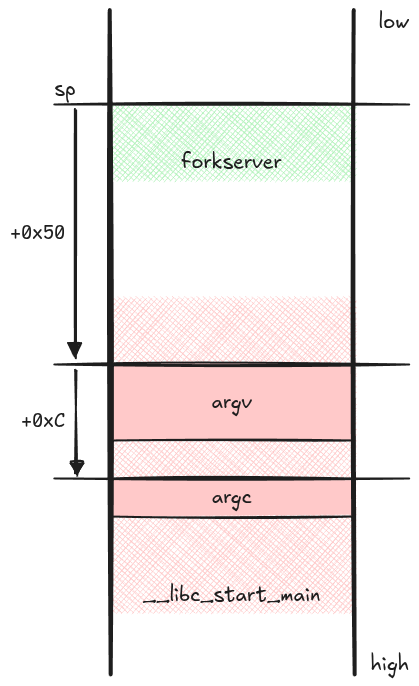
\includegraphics[width=0.25\textwidth]{img/fsrv-memlyt.png}
    \caption{forkserver Memory Layout}
    \label{fig:fsrv-memlyt}
\end{figure}
\fi